\documentclass[11pt]{article}
\usepackage{enumerate}
\usepackage{fullpage}
\usepackage{fancyhdr}
\usepackage{amsmath, amsfonts, amsthm, amssymb}
\usepackage{color}
\usepackage[]{graphicx}

\setlength{\parindent}{0pt}
\setlength{\parskip}{5pt plus 1pt}
\pagestyle{empty}

\def\indented#1{\list{}{}\item[]}
\let\indented=\endlist

\newcounter{questionCounter}
\newcounter{partCounter}[questionCounter]
\newenvironment{question}[2][\arabic{questionCounter}]{%
    \setcounter{partCounter}{0}%
    \vspace{.25in} \hrule \vspace{0.5em}%
        \noindent{\bf #2}%
    \vspace{0.8em} \hrule \vspace{.10in}%
    \addtocounter{questionCounter}{1}%
}{}
\renewenvironment{part}[1][\alph{partCounter}]{%
    \addtocounter{partCounter}{1}%
    \vspace{.10in}%
    \begin{indented}%
       {\bf (#1)} %
}{\end{indented}}

%%%%%%%%%%%%%%%%%%%%%%%HEADER%%%%%%%%%%%%%%%%%%%%%%%%%%%%%%
\newcommand{\myname}{Shashank Singh}
\newcommand{\myandrew}{sss1@andrew.cmu.edu}
\newcommand{\myclass}{86-595 Neural Data Analysis}
\newcommand{\myhwnum}{6}
\newcommand{\duedate}{Tuesday, December 4, 2012}
%%%%%%%%%%%%%%%%%%%%%%%%%%%%%%%%%%%%%%%%%%%%%%%%%%%%%%%%%%%

%%%%%%%%%%%%%%%%%%%%CONTENT MACROS%%%%%%%%%%%%%%%%%%%%%%%%%
\newcommand{\ans}[1]{\mbox{\fbox{$\displaystyle #1$}}} % box around an answer in math mode
\renewcommand{\qed}{\quad $\blacksquare$} % black QED square
\newcommand{\mqed}{\quad \blacksquare} % black QED square for use in math mode
\newcommand{\inv}{^{-1}} % inverse
\newcommand{\blambda}{\boldsymbol{\lambda}}
\newcommand{\br}{\mathbf{r}}
\newcommand{\bx}{\mathbf{x}}
\newcommand{\by}{\mathbf{y}}
\newcommand{\bff}{\mathbf{f}}
\newcommand{\bzero}{\mathbf{0}}
\newcommand{\N}{\mathbb{N}} % natural numbers
\newcommand{\Q}{\mathbb{Q}} % rational numbers
\newcommand{\R}{\mathbb{R}} % real numbers
\newcommand{\E}[1]{\mathsf{E}\left[#1\right]} % expected value
\newcommand{\Var}[1]{\mathsf{Var}\left[#1\right]} % variance
\newcommand{\Poisson}[1]{\operatorname{Poisson}\left(#1\right)} % Poisson distribution
\newcommand{\Exp}[1]{\operatorname{Exp}\left(#1\right)} % Exponential distribution
\newcommand{\U}[2]{\operatorname{U}\left(#1,#2\right)} % Uniform distribution
\newcommand{\Bern}[1]{\operatorname{Bernoulli}\left( #1 \right)} % Bernoulli distribution
\newcommand{\pr}[1]{\mathsf{P}\left( #1 \right)} % probability of event #1
\newcommand{\giv}{\, | \,} % \pr{A \giv B} is the probability of A given B
\newcommand{\argmax}{\operatornamewithlimits{argmax}}
\newcommand{\argmin}{\operatornamewithlimits{argmin}}
%%%%%%%%%%%%%%%%%%%%%%%%%%%%%%%%%%%%%%%%%%%%%%%%%%%%%%%%%%%

\begin{document}
\thispagestyle{plain}

{\Large Homework \myhwnum} \\
\myclass \\
Name: \myname \\
Email: \myandrew \\
Due: \duedate \\
\begin{question}{Problem 1}
Using the previous estimate as the prior will bias the next estimated velocity
toward the previous estimates, because the prior for each estimate will
include the product of all previous priors. As a result, earlier estimates
will play a significant role in later estimate, even after long periods of
time. Changes in velocity will be estimated more slowly and to a lesser degree
than they occur. As time progresses, this effect will compound, until the
estimator is no longer sensitive to changes in velocity, because the prior is
so strong, and the estimate will converge on a steady state velocity.
\end{question}

\begin{question}{Problem 2}
\begin{enumerate}[a.]
\item
See Figures~\ref{fig:2a1}, ~\ref{fig:2a2} and ~\ref{fig:2a3}. Blue plots are
$x$-coordinates, and red plots are $y$-coordinates. Solid lines are actual,
velocities and dotted lines are predicted velocities.
\begin{figure}[h]
\begin{center}
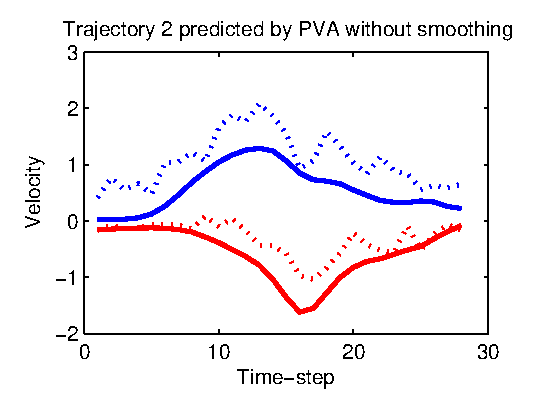
\includegraphics[width=0.46\textwidth]{2a1}
\end{center}
\caption{No smoothing.}
\label{fig:2a1}
\end{figure}
\begin{figure}[h]
\begin{center}
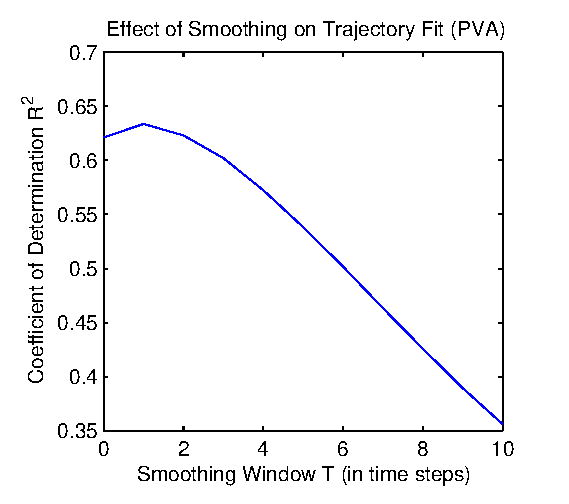
\includegraphics[width=0.46\textwidth]{2a2}
\end{center}
\caption{$R^2$ value for each smoothing window size}
\label{fig:2a2}
\end{figure}
\begin{figure}[h]
\begin{center}
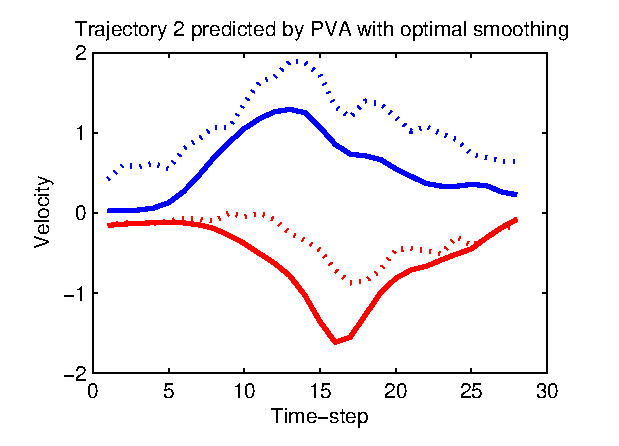
\includegraphics[width=0.46\textwidth]{2a3}
\end{center}
\caption{Optimal smoothing}
\label{fig:2a3}
\end{figure}

\item
See Figures~\ref{fig:2b1}, ~\ref{fig:2b2} and ~\ref{fig:2b3}.
\begin{figure}[h]
\begin{center}
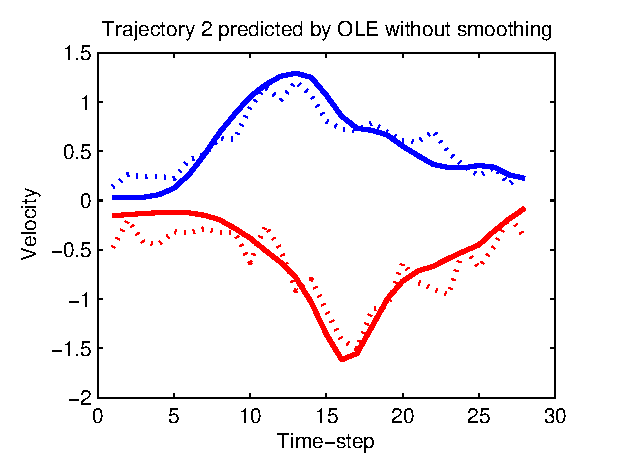
\includegraphics[width=0.46\textwidth]{2b1}
\end{center}
\caption{No smoothing.}
\label{fig:2b1}
\end{figure}
\begin{figure}[h]
\begin{center}
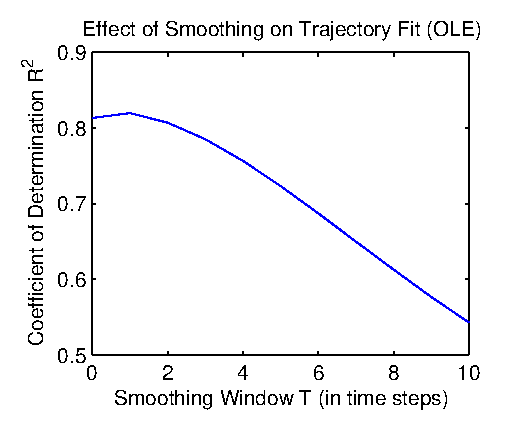
\includegraphics[width=0.46\textwidth]{2b2}
\end{center}
\caption{$R^2$ value for each smoothing window size}
\label{fig:2b2}
\end{figure}
\begin{figure}[h]
\begin{center}
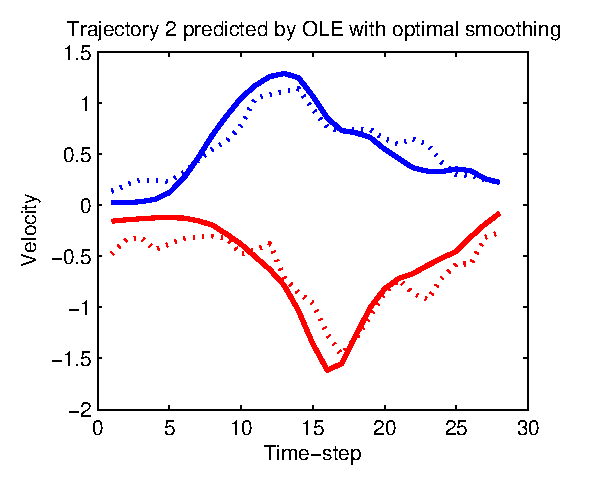
\includegraphics[width=0.46\textwidth]{2b3}
\end{center}
\caption{Optimal smoothing}
\label{fig:2b3}
\end{figure}

\item File sent in email.

\end{enumerate}
\end{question}

\newpage
\begin{question}{Problem 3}
Question 1 (concerning Kalman filters) seemed pretty apparent after thinking
for a few minutes about how the estimator would work. Of the programming
section, part 2a. took most of the time, since PVA has a few steps. Part 2b,
on the other hand, was just one line of code on top of a few lines for
smoothing, so that, after implementing smoothing for part 2a., part 2b., took
only a couple of minutes.

Since I wasn't able to spend much time on part 2c., I didn't end up
implementing a Kalman filter or a Poisson MLE estimator and just used my OLE
implementation from part 2b. But I imagine that, if I had more time,
trying to implement a better estimator would have been informative.
I might have liked a bit more theory to help understand the details of OLE and
Kalman filters, or perhaps to derive the MLE hinted at in part 2c.
\end{question}
\newpage
\begin{question}{Code}
PVA implementation:
\begin{verbatim}
function pred_traj = PVA(spikes, cosine_fit, dt, T)

  [neurons times] = size(spikes);
  b0 = cosine_fit.b0s;
  B = cosine_fit.Bs;

  % use Euclidean norm of each b as modulation depth
  mod = sqrt(diag(B * B'));

  % normalize firing rates at each time step
  normed = zeros(size(spikes));
  for time = 1:times
    normed(:,time) = (spikes(:,time) - b0) ./ mod;
  end

  % smooth firing rates; traverse normed backward
  for time = times:-1:1
    normed(:,time) = mean(normed(:,max(1,time - T):time), 2);
  end

  % pool firing rates at each time step
  pred_traj = zeros(times, 2);
  for time = 1:times
    pred_traj(time, :) = (normed(:,time)') * B / neurons;
  end
end
\end{verbatim}

OLE implementation:
\begin{verbatim}
function pred_traj = OLE(spikes, cosine_fit, dt, T)
  [~, times] = size(spikes);
  B = cosine_fit.Bs;
  sigma = cosine_fit.sigma;

  % smooth firing rates; traverse spikes backward
  for time = times:-1:1
    spikes(:,time) = mean(spikes(:,max(1,time - T):time), 2);
  end

  % decoding matrix
  G = inv\left( B') * inv(sigma) * B) * (B') * inv(sigma);

  pred_traj = (G * spikes)';
end
\end{verbatim}
\end{question}
\end{document}
